\documentclass{standalone}
\usepackage{tikz}
\usepackage{pgfplots}

\pgfplotsset{compat = newest}

\definecolor{color_green1}{RGB}{160,240,160}
\definecolor{color_green2}{RGB}{0,180,0}
\definecolor{color_green3}{RGB}{0,100,0}
\def\m{2} % mean
\def\o{0.2} % variance
\def\oo{1} % variance
\def\ooo{5} % variance

\begin{document}
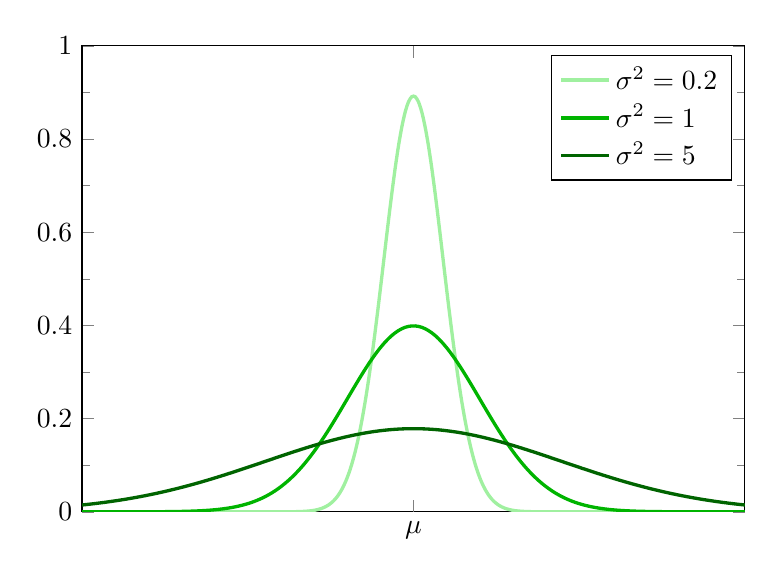
\begin{tikzpicture}
  \begin{axis}[
      xmin = 2 - 5, xmax = 2 + 5, %
      ymin = 0, ymax = 1, %
      x label style={at={(axis description cs:0.9,-0.025)},anchor=north},
      y label style={at={(axis description cs:-0.075,0.9)},anchor=south},
      xtick = {-4}, % A random number (out of the graphic), which is necessary (it cannot be: xtick = {})
      extra x ticks = {2},
      extra x tick labels={$\mu$},
      minor tick num = 1, %Is the number of ticks between major ticks.
      major grid style = {lightgray}, %Changes the color and stroke of the major grid.
      minor grid style = {lightgray!25}, %Changes the color and stroke of the minor grid.
      width = 10cm, %sets the width of the figure
      height = 7.5cm,  %sets the height of the figure
      xlabel = {}, %
      ylabel = {}, %
      legend cell align = {left}, %
      legend style={} % position of the legend box and anchor is the point on the box to be fitted exactly at the point of cs:<>,<>. Options are anchor=center,south west,south east,north west,north east,north,south,west... Example: legend style={at={(axis cs:0,-0.5)},anchor=center}
    ]
    \addplot[
      domain=-3:7, %Domain of the fucntion
      samples=200, %This parameter determines the number of point to be plotted for the function, while bigger the number better looks the function.
      smooth, %f we use this option, the compiler makes an interpolation between the point plotted to get a soft appearance for the function.
      very thick, %Stroke of the function. Options: ultra thin, very thin, thin, semithick, thick, very thick, ultra thick.
      color_green1 %Color of the function.
    ]{1/(2*pi*\o)^(1/2)*exp{-(x-\m)^2/(2*\o)}};
    \addplot[
      domain=-3:7, %Domain of the fucntion
      samples=200, %This parameter determines the number of point to be plotted for the function, while bigger the number better looks the function.
      smooth, %f we use this option, the compiler makes an interpolation between the point plotted to get a soft appearance for the function.
      very thick, %Stroke of the function. Options: ultra thin, very thin, thin, semithick, thick, very thick, ultra thick.
      color_green2 %Color of the function.
    ]{1/(2*pi*\oo)^(1/2)*exp{-(x-\m)^2/(2*\oo)}};
    \addplot[
      domain=-3:7, %Domain of the fucntion
      samples=200, %This parameter determines the number of point to be plotted for the function, while bigger the number better looks the function.
      smooth, %f we use this option, the compiler makes an interpolation between the point plotted to get a soft appearance for the function.
      very thick, %Stroke of the function. Options: ultra thin, very thin, thin, semithick, thick, very thick, ultra thick.
      color_green3 %Color of the function.
    ]{1/(2*pi*\ooo)^(1/2)*exp{-(x-\m)^2/(2*\ooo)}};
    \legend{$\sigma^2=\o$,$\sigma^2=\oo$,$\sigma^2=\ooo$}
  \end{axis}
\end{tikzpicture}
\end{document}